% !TEX root = 20250826_COMULIS_microCT.tex

\usetheme[language=english]{ubbeamer2023}

\title{\uct and image analysis}
\subtitle{\href{https://www.ana.unibe.ch/weiterbildung/comulis_training_school/}{COMULIS Training School - Imaging Across Scales}}
\author{David Haberthür}
\institute{Institute of Anatomy}
\date{August 26, 2025}

% Some often used abbreviations/commands
\newcommand{\everyframe}{1}% use only every nth frame for the animations
\newcommand{\imagewidth}{\columnwidth}% set global image width
\newcommand{\imageheight}{0.7\paperheight}% set global image heidht
\newlength\imagescale% needed for scalebars
\newcommand{\uct}{{\textmu}CT\xspace}% make our life easier
\newcommand{\eg}{e.\,g.\xspace}%
\newcommand{\ie}{i.\,e.\xspace}%

\usepackage[backend=biber,
	style=numeric,
	url=false,
	isbn=true,
	maxnames=1,
	sorting=none]{biblatex}
\addbibresource{../../Documents/library.bib}% FastSSD, Windows or Mac works (on Linux/FastSSD we generated a 'Document' folder at the correct level and `ln -s ~/P/Documents/library.bib .` to it)
\usepackage{microtype}
\usepackage[detect-all=true,
	range-phrase=--,
	range-units=single,
	per-mode=symbol,
	per-symbol=/]{siunitx}
\usepackage{xspace}
\usepackage{csquotes}
\usepackage{pgfplotstable}
 	\pgfplotsset{compat=newest}
\usepackage{booktabs}
\usepackage{colortbl}
\usepackage{ccicons}
\usepackage{animate}
\usepackage{fontawesome5}
\usepackage{tikz}
% 	\usetikzlibrary{spy}
 	\tikzset{shadowed/.style={preaction={transform canvas={shift={(1pt,-1pt)}},draw=ubRed}}}
\usepackage{standalone}
\usepackage{listings}
	\lstset{frame=single,
		backgroundcolor = \color{ubGrey!38.2},
		basicstyle=\tiny\ttfamily
		}
\usepackage{shadowtext}% for the shadowed scalebar
	\shadowoffset{1pt}
	\shadowcolor{ubRed}
\usepackage{qrcode}
\usepackage{mathastext}

% Define complementary colors to ubRed=e4003c, which is defined in the .sty file
% https://duckduckgo.com/?t=lm&q=html+e4003c&ia=answer
\definecolor{ubRedComplementary}{HTML}{00E3A6}


% \usepackage{pgfplots}

% \usepackage{standalone}


% \usepackage[absolute,overlay]{textpos}%for the \source{} command
% \usepackage[missing=main]{gitinfo2}% GitHub Actions don't pull in the commit hash, so we just show `main`


% \usepackage[version=4]{mhchem}






% \usepackage{multirow}
% \usepackage{mathastext}

% % change tikz font to slide font
% % https://tex.stackexchange.com/a/33329/828
% \usepackage[eulergreek]{sansmath}
% 	\pgfplotsset{tick label style = {font=\sansmath\sffamily},
% 		every axis label = {font=\sansmath\sffamily},
% 		legend style = {font=\sansmath\sffamily},
% 		label style = {font=\sansmath\sffamily}
% 		}

% % Globally thicker lines in with tikz
% % https://tex.stackexchange.com/a/206769/828
% \tikzset{every picture/.style={thick}}

% Acknowledge images just below them
% Based on https://tex.stackexchange.com/a/282637/828
\newcommand{\source}[2]{%
	% Print out (short) link under image, with small text
	\raisebox{-1ex}{%
		\makebox[0pt][r]{%
			\usebeamerfont{footline}\href{http://#1}{#1} #2%
			}%
		}%
	}%
\newcommand{\sourcelink}[3]{%
	% Make the source command an \href{link}{text}
	\raisebox{-1ex}{%
		\makebox[0pt][r]{%
			\usebeamerfont{footline}\href{http://#1}{#2}, #3%
			}%
		}%
	}%
\newcommand{\sourcecite}[2]{%
	% Cite (an image from) a reference
	\raisebox{-1ex}{%
		\makebox[0pt][r]{%
			\usebeamerfont{footline}From \cite{#1}, #2%
			}%
		}%
	}%
\newcommand{\sourceqr}[1]{%
	% Cite (an image from) a (long) URL with a QR code
	\raisebox{0.63cm}{%
		\makebox[0pt][l]{%
			\qrcode[height=1.5cm]{#1}%
			}%
		}%
	}%	

% % Define us a custom footer *with* progress bar, based on https://tex.stackexchange.com/a/59749/828
% \makeatletter
% \def\progressbar@progressbar{}% the progress bar
% \newcount\progressbar@tmpcounta% auxiliary counter
% \newcount\progressbar@tmpcountb% auxiliary counter
% \newdimen\progressbar@pbht%progressbar height
% \newdimen\progressbar@pbwd%progressbar width
% \newdimen\progressbar@rcircle% radius for the circle
% \newdimen\progressbar@tmpdim% auxiliary dimension
% \progressbar@pbwd=0.85\linewidth%
% \progressbar@rcircle=1.5pt%
% \def\progressbar@progressbar{%
% 	\progressbar@tmpcounta=\insertframenumber%
% 	\progressbar@tmpcountb=\inserttotalframenumber%
% 	\progressbar@tmpdim=\progressbar@pbwd%
% 	\multiply\progressbar@tmpdim by \progressbar@tmpcounta%
% 	\divide\progressbar@tmpdim by \progressbar@tmpcountb%
% 	\par%
% 	\mode<beamer>{\begin{tikzpicture}%
% 		\draw[ubGrey] (0,0) -- ++ (\progressbar@pbwd,0);%
% 		\draw[draw=ubRed,fill=ubGrey]
% (\the\dimexpr\progressbar@tmpdim-\progressbar@rcircle\relax,.5\progressbar@pbht
% ) circle (\progressbar@rcircle);%
% 	\end{tikzpicture}%
% 	\hfill}bit.ly/cmls\xspace|\xspace%
% 	v.
% \href{https://github.com/habi/Talk.2025.COMULIS/commit/\gitHash}{\gitAbbrevHash
% }\xspace|\xspace%
% 	p.\xspace\insertframenumber/\inserttotalframenumber%
% 	\hspace*{4ex}%
% 	\vspace{0.5ex}%
% }

% \addtobeamertemplate{footline}{}%
% {%
% 	\begin{beamercolorbox}[wd=\paperwidth,center]{white}%
% 		\progressbar@progressbar%
% 	\end{beamercolorbox}%
% }%
% \makeatother

% % Format bibliography for beamer
% % http://tex.stackexchange.com/a/10686/828
% \renewbibmacro{in:}{}
% % http://tex.stackexchange.com/a/13076/828
% \AtEveryBibitem{%
% 	\clearfield{journaltitle}
% 	\clearfield{pages}
% 	\clearfield{volume}
% 	\clearfield{number}
% 	\clearname{editor}
% 	\clearfield{issn}
% 	\clearfield{year}
% }
% % No parentheses around the (now empty) year: https://tex.stackexchange.com/a/147537/828
% \renewcommand{\bibopenparen}{\addcomma\addspace}
% \renewcommand{\bibcloseparen}{\addcomma\addspace}

% % Redefine \footcite based on https://tex.stackexchange.com/a/453528/828
% \DeclareCiteCommand{\footcite}[\mkbibfootnote]{%
% 	\usebibmacro{prenote}}{%
% 		\printnames[family-given]{labelname}%
% 		\newunit%
% 		\addcolon\space\thefield{url}% print only the field, but not the name of the field
% 		\newunit%
% 		\printlabeldateextra%
% 	}{\addsemicolon\space}{%
% 		\usebibmacro{postnote}%
% 	}%

% % References as footnotes at the bottom of the slides
% % https://tex.stackexchange.com/a/368760/828
% \makeatletter
% \renewcommand\@makefnmark{\xspace\hbox{\usebeamercolor[fg]{footnote mark}\usebeamerfont*{footnote mark}[\@thefnmark]}}
% \renewcommand\@makefntext[1]{\tiny{\usebeamercolor[fg]{footnote mark}\usebeamerfont*{footnote mark}[\@thefnmark]}\enspace\usebeamerfont*{footnote} #1}
% \makeatother

% Show current section at begin of sections, but only in presentation mode
\mode<beamer>{%
	\AtBeginSection[]{%
		\begin{frame}{Contents}%
			\tableofcontents[currentsection,currentsubsection,hideothersubsections]%
		\end{frame}%
	}%
}

\begin{document}

\begin{frame}
	\titlepage%
	\begin{flushright}%
		\mode<beamer>{\qrcode[height=4cm]{https://habi.github.io/Talk.2025.COMULIS/20250826_COMULIS_microCT_handout.pdf}}%
	\end{flushright}%
\end{frame}

\begin{frame}
	\frametitle{Grüessech!}
	\begin{itemize}
		\item David Haberthür
		\begin{itemize}
			\item Physicist by trade
			\item \href{https://boris.unibe.ch/2619/}{PhD in high resolution imaging of the lung}, Institute of Anatomy, University of Bern, Switzerland
			\item Post-Doc I: Tomographic imaging at \href{https://www.psi.ch/sls/tomcat/}{TOMCAT}, \href{https://www.psi.ch/sls/}{Swiss Light Source}, \href{https://www.psi.ch/}{Paul Scherrer Institute}, Switzerland and working on the detector of the \href{http://globaldiagnostix.org}{GlobalDiagnostiX} project
			\item Post-Doc II \& currently: Tomographic imaging in the \href{https://www.ana.unibe.ch/forschung/mikroct/research/}{\uct group}, Institute of Anatomy, University of Bern, Switzerland
		\end{itemize}
	\end{itemize}
\end{frame}

\begin{frame}
	\frametitle{\uct-group}
	\begin{columns}
		\begin{column}{0.6177\linewidth}
			\begin{itemize}
				\item microangioCT~\cite{Hlushchuk2018} in heart, musculature~\cite{Nording2021} bones~\cite{Haberthuer2025}, (mouse) brain~\cite{Hlushchuk2020}, (human) nerve scaffolds~\cite{Wuthrich2020}, (human) skin flaps~\cite{Zubler2021} and tumors\cite{Fernandez2025}.
				\item (Lung) tumor detection and metastasis classification~\cite{Trappetti2021}
				\item Collaborations with museums~\cite{Bochud2021} and scientist at UniBe~\cite{Halm2021} to scan a wide range of specimens~\cite{MesserliAaldijk2020,Haberthuer2023}
				\item Automate \emph{all} the things!~\cite{Haberthuer2021, Haberthuer2023}
			\end{itemize}
		\end{column}%
		\begin{column}{0.3822\linewidth}%
			\centering%
			\includegraphics<1|handout:0>[width=\imagewidth]{./images/1172}%
			\only<1|handout:0>{\source{brukersupport.com}{}}%
			\includegraphics<2|handout:1>[width=\imagewidth]{./images/1272}%
			\only<2|handout:1>{\source{bruker.com/skyscan1272}{}}%
			\includegraphics<3|handout:0>[width=\imagewidth]{./images/2214}%
			\only<3|handout:0>{\source{bruker.com/skyscan2214}{}}%
		\end{column}%
	\end{columns}%
\end{frame}

\begin{frame}{Contents}
	\tableofcontents
\end{frame}

\section{Overview}
\begin{frame}
	\frametitle{Overview}
	\centering
	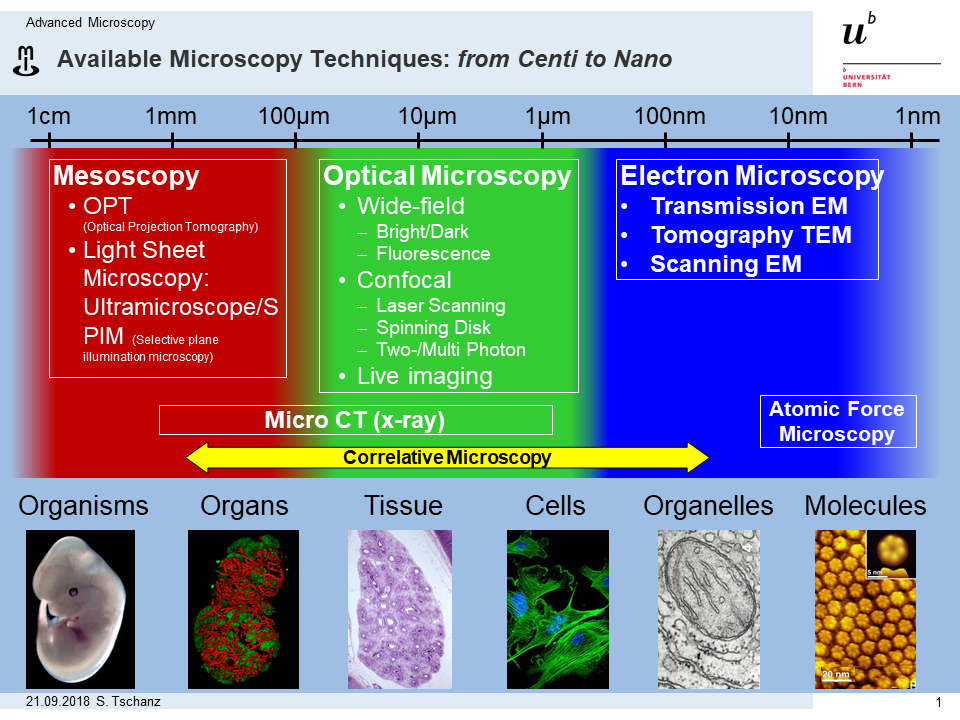
\includegraphics[height=\imageheight]{./images/MIC-AM_techniques}%
	\sourcelink{https://anatomie.unibe.ch/tschanz}{Stefan Tschanz}{with permission}%
\end{frame}

\subsection{Tomography}
\begin{frame}
	\frametitle{What is happening?}
	\begin{columns}%
		\begin{column}{0.3822\linewidth}%
			Basic components of computer tomography devices:
			\begin{itemize}
				\item an X-ray source
				\item something to look through
				\item a detector
			\end{itemize}
		\end{column}%
		\begin{column}{0.6177\linewidth}%
			\centering%
			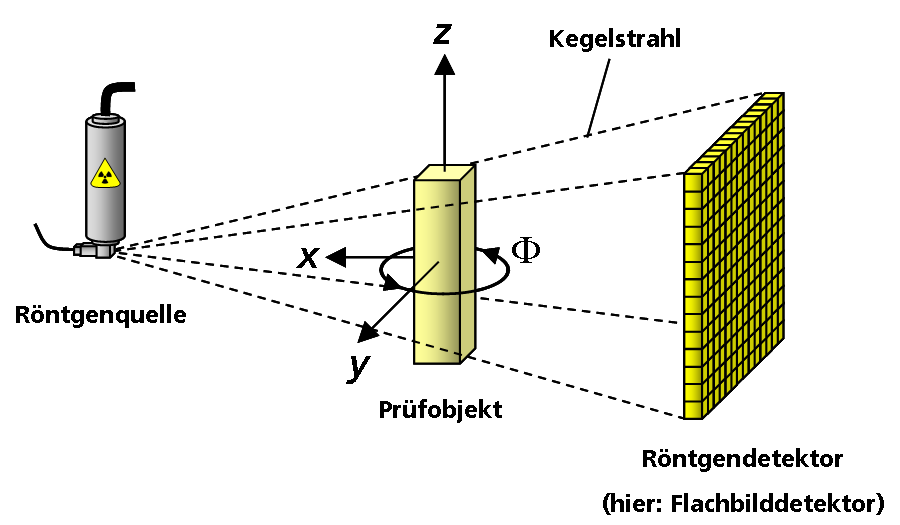
\includegraphics[width=\imagewidth]{./images/3D_Computed_Tomography}%
			\source{w.wiki/7g3}{\ccbysa}%
		\end{column}%
	\end{columns}%
\end{frame}

\begin{frame}
	\frametitle{Machinery}
	\begin{columns}
		\begin{column}{0.5\textwidth}
			\centering%
			\documentclass{standalone}%
% Draw the setup where the source and detector move, e.g. classic CT
% With help from https://tex.stackexchange.com/q/515519/828
\usepackage{fontawesome5}
\usepackage{ifthen}
\ifthenelse{\isundefined{\everyframe}}{%
	% If we're compiling this file via \input, then we already defined some things
	% In the other case, we need to define them
	\usepackage{tikz}
	\usepackage{animate}
	\newcommand{\everyframe}{5}
	\definecolor{ubRed}{HTML}{e4003c}%
	\definecolor{ubGrey}{HTML}{646363}%
	% split complementary images from https://www.sessions.edu/color-calculator/
	\definecolor{ubRedComplementary}{HTML}{2EE600}
	}{}
\begin{document}
\begin{animateinline}[loop,every=\everyframe]{25}
	\multiframe{90}{n=1+4}{%
		\begin{tikzpicture}[scale=1.25]
			\pgfdeclarelayer{background}
			\pgfsetlayers{background,main}
			%Help lines used to setup the animation (set to semitransparent), drawing them transparent in the presentation forces a consistent size
			\begin{pgfonlayer}{background}
				\draw[ubGrey,transparent,help lines,step=5mm] (-2.05,-2.05) grid (2.05,2.05);
			\end{pgfonlayer}
			% Stuff that stays put
			\node[ubRedComplementary] at (0,0) (sample) {\Huge\faUser};
			% Stuff that moves
				\begin{scope}[rotate around={\n:(sample)}]
				% Rotation arc
				\draw[->, thick,line cap=rect] (1.5,0) arc [start angle=0, end angle=180, radius=1.5];
				\draw[->, thick,line cap=rect] (-1.5,0) arc [start angle=-180, end angle=0, radius=1.5];
				% Source
				\fill[ubRed] (-0.25,1.5) rectangle node (source) {} +(0.5,0.5);
				\draw[fill=yellow] (0,1.75) circle (0.2);
				\node at (0,1.735) (radiation) {\small\faRadiation};
				% Detector and detector edges
				\fill[gray] (-0.5,-1.75) rectangle node (detector) {} +(1,0.25);
				\coordinate (dl) at (-0.45,-1.75);
				\coordinate (dr) at (0.45,-1.75);
				% X-ray cone
				\begin{pgfonlayer}{background}
					\fill[gray,semitransparent] (source.center) -- (dl) -- (dr) -- cycle;
				\end{pgfonlayer}
				\end{scope}
		\end{tikzpicture}
	}
\end{animateinline}
\end{document}
%
			\pause%
		\end{column}%
		\begin{column}{0.5\textwidth}%
			\centering%
			% "List" the LR, normal and HR animations in a weird order here, to display them logically side-by-side in the handout
			\only<3|handout:1>{\documentclass{standalone}%
% Draw the setup where the source and detector move, e.g. classic CT
% With help from https://tex.stackexchange.com/q/515519/828
\usepackage{fontawesome5}
\usepackage{ifthen}
\ifthenelse{\isundefined{\everyframe}}{%
	% If we're compiling this file via \input, then we already defined some things
	% In the other case, we need to define them
	\usepackage{tikz}
	\usepackage{animate}
	\newcommand{\everyframe}{5}
	\definecolor{ubRed}{HTML}{e4003c}%
	\definecolor{ubGrey}{HTML}{646363}%
	% split complementary images from https://www.sessions.edu/color-calculator/
	\definecolor{ubRedComplementary}{HTML}{2EE600}
	}{}
\begin{document}
\begin{animateinline}[loop,every=\everyframe]{25}
	\multiframe{90}{n=1+4}{%
		\begin{tikzpicture}[scale=1.25]
			\pgfdeclarelayer{background}
			\pgfsetlayers{background,main}
			%Help lines used to setup the animation (set to semitransparent), drawing them transparent in the presentation forces a consistent size
			\begin{pgfonlayer}{background}
				\draw[ubGrey,transparent,help lines,step=5mm] (-0.75,-1.25) grid (0.75,1.5);
			\end{pgfonlayer}
			% Stuff that stays put
			% Source
			\fill[ubRed] (-0.25,1) rectangle node (source) {} +(0.5,0.5);
			\draw[fill=yellow] (0,1.25) circle (0.2);
			\node at (0,1.235) (radiation) {\small\faRadiation};
			% Detector and detector edges
			\fill[gray] (-0.5,-1.25) rectangle node (detector) {} +(1,0.25);
			\coordinate (dl) at (-0.45,-1);
			\coordinate (dr) at (0.45,-1);
			% X-ray cone
			\begin{pgfonlayer}{background}
				\fill[gray,semitransparent] (source.center) -- (dl) -- (dr) -- cycle;
			\end{pgfonlayer}
			% Stuff that moves
				\begin{scope}[rotate around={\n:(0,-0.5)}]
				% Rotation arc
				\draw[->, thick,line cap=rect] (0.618,-0.5) arc [start angle=0, end angle=180, radius=0.618];
				\draw[->, thick,line cap=rect] (-0.618,-0.5) arc [start angle=-180, end angle=0, radius=0.618];
				% Sample
				\node[ubRedComplementary] at (0,-0.5) (sample) {\rotatebox{\n}{\huge\faFish}};
				\end{scope}
		\end{tikzpicture}
	}
\end{animateinline}
\end{document}
}%
			\only<1-2|handout:1>{\documentclass{standalone}%
% Draw the setup where the source and detector move, e.g. classic CT
% With help from https://tex.stackexchange.com/q/515519/828
\usepackage{fontawesome5}
\usepackage{ifthen}
\ifthenelse{\isundefined{\everyframe}}{%
	% If we're compiling this file via \input, then we already defined some things
	% In the other case, we need to define them
	\usepackage{tikz}
	\usepackage{animate}
	\newcommand{\everyframe}{5}
	\definecolor{ubRed}{HTML}{e4003c}%
	\definecolor{ubGrey}{HTML}{646363}%
	% split complementary images from https://www.sessions.edu/color-calculator/
	\definecolor{ubRedComplementary}{HTML}{2EE600}
	}{}
\begin{document}
\begin{animateinline}[loop,every=\everyframe]{25}
	\multiframe{90}{n=1+4}{%
		\begin{tikzpicture}[scale=1.25]
			\pgfdeclarelayer{background}
			\pgfsetlayers{background,main}
			%Help lines used to setup the animation (set to semitransparent), drawing them transparent in the presentation forces a consistent size
			\begin{pgfonlayer}{background}
				\draw[ubGrey,transparent,help lines,step=5mm] (-0.75,-1.25) grid (0.75,1.5);
			\end{pgfonlayer}
			% Stuff that stays put
			% Source
			\fill[ubRed] (-0.25,1) rectangle node (source) {} +(0.5,0.5);
			\draw[fill=yellow] (0,1.25) circle (0.2);
			\node at (0,1.235) (radiation) {\small\faRadiation};
			% Detector and detector edges
			\fill[gray] (-0.5,-1.25) rectangle node (detector) {} +(1,0.25);
			\coordinate (dl) at (-0.45,-1);
			\coordinate (dr) at (0.45,-1);
			% X-ray cone
			\begin{pgfonlayer}{background}
				\fill[gray,semitransparent] (source.center) -- (dl) -- (dr) -- cycle;
			\end{pgfonlayer}
			% Stuff that moves
				\begin{scope}[rotate around={\n:(0,0)}]
				% Rotation arc
				\draw[->, thick,line cap=rect] (0.618,0) arc [start angle=0, end angle=180, radius=0.618];
				\draw[->, thick,line cap=rect] (-0.618,0) arc [start angle=-180, end angle=0, radius=0.618];
				% Sample
				\node[ubRedComplementary] at (0,0) (sample) {\rotatebox{\n}{\normalsize\faFish}};
				\end{scope}
		\end{tikzpicture}
	}
\end{animateinline}
\end{document}
}%
			\only<4|handout:1>{\documentclass{standalone}%
% Draw the setup where the source and detector move, e.g. classic CT
% With help from https://tex.stackexchange.com/q/515519/828
\usepackage{fontawesome5}
\usepackage{ifthen}
\ifthenelse{\isundefined{\everyframe}}{%
	% If we're compiling this file via \input, then we already defined some things
	% In the other case, we need to define them
	\usepackage{tikz}
	\usepackage{animate}
	\newcommand{\everyframe}{5}
	\definecolor{ubRed}{HTML}{e4003c}%
	\definecolor{ubGrey}{HTML}{646363}%
	% split complementary images from https://www.sessions.edu/color-calculator/
	\definecolor{ubRedComplementary}{HTML}{2EE600}
	}{}
\begin{document}
\begin{animateinline}[loop,every=\everyframe]{25}
	\multiframe{90}{n=1+4}{%
		\begin{tikzpicture}[scale=1.25]
			\pgfdeclarelayer{background}
			\pgfsetlayers{background,main}
			%Help lines used to setup the animation (set to semitransparent), drawing them transparent in the presentation forces a consistent size
			\begin{pgfonlayer}{background}
				\draw[ubGrey,transparent,help lines,step=5mm] (-0.75,-1.25) grid (0.75,1.5);
			\end{pgfonlayer}
			% Stuff that stays put
			% Source
			\fill[ubRed] (-0.25,1) rectangle node (source) {} +(0.5,0.5);
			\draw[fill=yellow] (0,1.25) circle (0.2);
			\node at (0,1.235) (radiation) {\small\faRadiation};
			% Detector and detector edges
			\fill[gray] (-0.5,-1.25) rectangle node (detector) {} +(1,0.25);
			\coordinate (dl) at (-0.45,-1);
			\coordinate (dr) at (0.45,-1);
			% X-ray cone
			\begin{pgfonlayer}{background}
				\fill[gray,semitransparent] (source.center) -- (dl) -- (dr) -- cycle;
			\end{pgfonlayer}
			% Stuff that moves
				\begin{scope}[rotate around={\n:(0,0.5)}]
				% Rotation arc
				\draw[->, thick,line cap=rect] (0.618,0.5) arc [start angle=0, end angle=180, radius=0.618];
				\draw[->, thick,line cap=rect] (-0.618,0.5) arc [start angle=-180, end angle=0, radius=0.618];
				% Sample
				\node[ubRedComplementary] at (0,0.5) (sample) {\rotatebox{\n}{\tiny\faFish}};
				\end{scope}
		\end{tikzpicture}
	}
\end{animateinline}
\end{document}
}%
		\end{column}
	\end{columns}
\end{frame}

\begin{frame}[allowframebreaks]
	\frametitle{Acquisition}
	\centering
	% Movie frames generated with https://github.com/habi/Lecture.Microtomography/blob/master/Notebooks/FromProjectionsToReconstructions.ipynb
	\mode<beamer>{\animategraphics[autoplay,loop,height=\imageheight,every=\everyframe]{24}{./movies/scan/projections/KP-TNIKWT02_240_projections_of_940_800_px_}{000}{313}}
	\mode<handout>{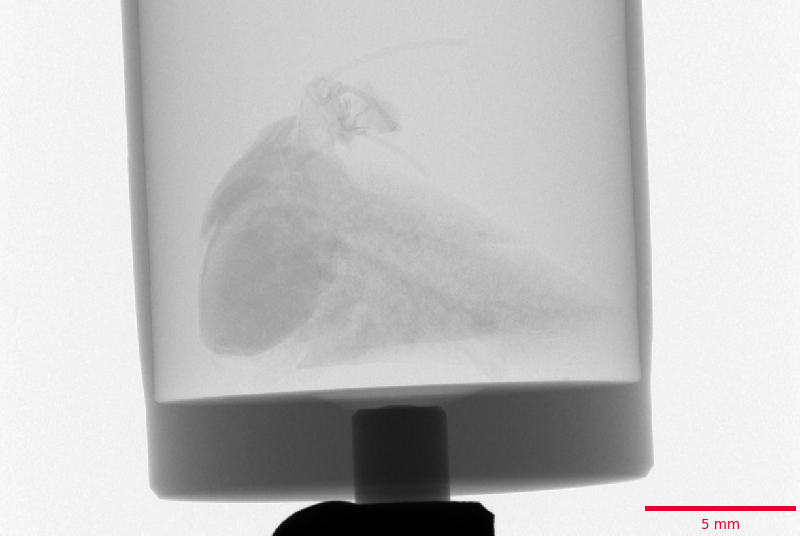
\includegraphics[height=\imageheight]{./movies/scan/projections/KP-TNIKWT02_240_projections_of_940_800_px_000}}
% \end{frame}

% \begin{frame}
% 	\frametitle{Acquisition}
% 	\centering
	% Movie downloaded from https://sites.google.com/a/fulbrightmail.org/kesnersmedicalphysics/home/education/3d-image-reconstruction-explained-with-animated-gifs, sligthly cropped in ImageJ, saved out and PNG images and piped through oxipng
	\mode<beamer>{\animategraphics[autoplay,palindrome,height=\imageheight,every=\everyframe]{5}{./movies/scan/acquisition/TOMO_gif_CT_signed00}{00}{91}\sourceqr{https://sites.google.com/a/fulbrightmail.org/kesnersmedicalphysics/home/education/3d-image-reconstruction-explained-with-animated-gifs}}%
	\mode<handout>{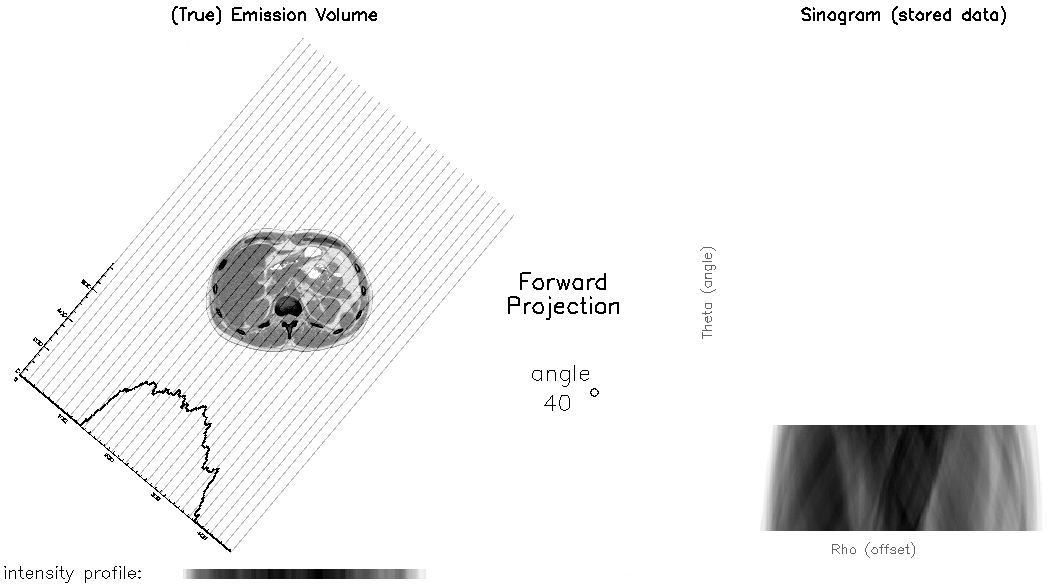
\includegraphics[height=\imageheight]{./movies/scan/acquisition/TOMO_gif_CT_signed0020}\sourceqr{https://sites.google.com/a/fulbrightmail.org/kesnersmedicalphysics/home/education/3d-image-reconstruction-explained-with-animated-gifs}}%
% \end{frame}

% \begin{frame}
% 	\frametitle{Projections}
	\begin{itemize}
		\item A (micro-focus) x-ray source illuminates the object
		\item The x-rays penetrate the sample and are attenuated
		\item A scintillator converts the x-rays to visible light
		\item A (planar) x-ray detector collects (magnified) projection images.
		\item The projections are recorded on disk
	\end{itemize}
\end{frame}

\begin{frame}[allowframebreaks]
	\frametitle{Reconstructions}
	\centering
	% Movie downloaded from https://sites.google.com/a/fulbrightmail.org/kesnersmedicalphysics/home/education/3d-image-reconstruction-explained-with-animated-gifs, sligthly cropped in ImageJ, saved out and PNG images and piped through oxipng
	\mode<beamer>{\animategraphics[autoplay,palindrome,height=\imageheight,every=\everyframe]{24}{./movies/scan/sinogram/TOMO_FBP_gif_CT_signed00}{00}{4}\sourceqr{https://sites.google.com/a/fulbrightmail.org/kesnersmedicalphysics/home/education/3d-image-reconstruction-explained-with-animated-gifs}}%
	\mode<handout>{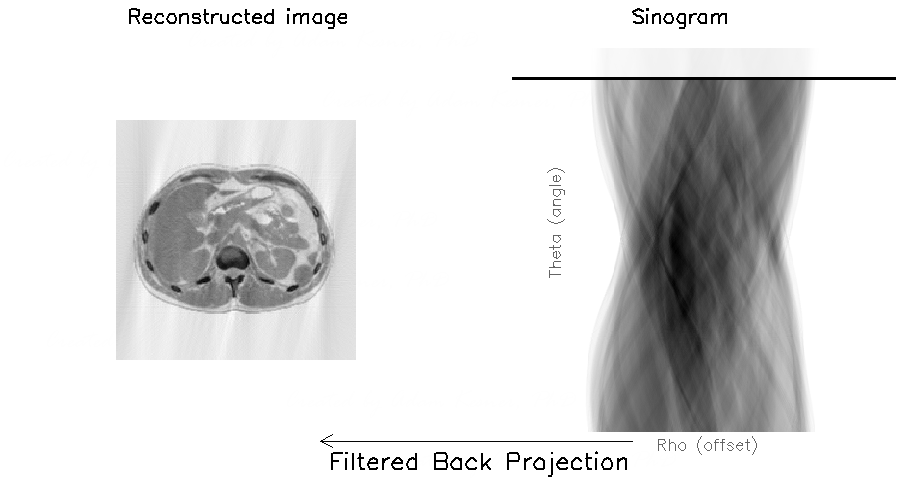
\includegraphics[height=\imageheight]{./movies/scan/sinogram/TOMO_FBP_gif_CT_signed0055}\sourceqr{https://sites.google.com/a/fulbrightmail.org/kesnersmedicalphysics/home/education/3d-image-reconstruction-explained-with-animated-gifs}}%
	
% \end{frame}

% \begin{frame}
% 	\frametitle{Reconstructions}
% 	\centering
	% Movie frames generated with https://github.com/habi/Lecture.Microtomography/blob/master/Notebooks/FromProjectionsToReconstructions.ipynb
	\mode<beamer>{\animategraphics[autoplay,palindrome,height=\imageheight,every=\everyframe]{24}{./movies/scan/reconstructions/KP-TNIKWT02_240_reconstructions_of_556_800_px_}{000}{277}}
	\mode<handout>{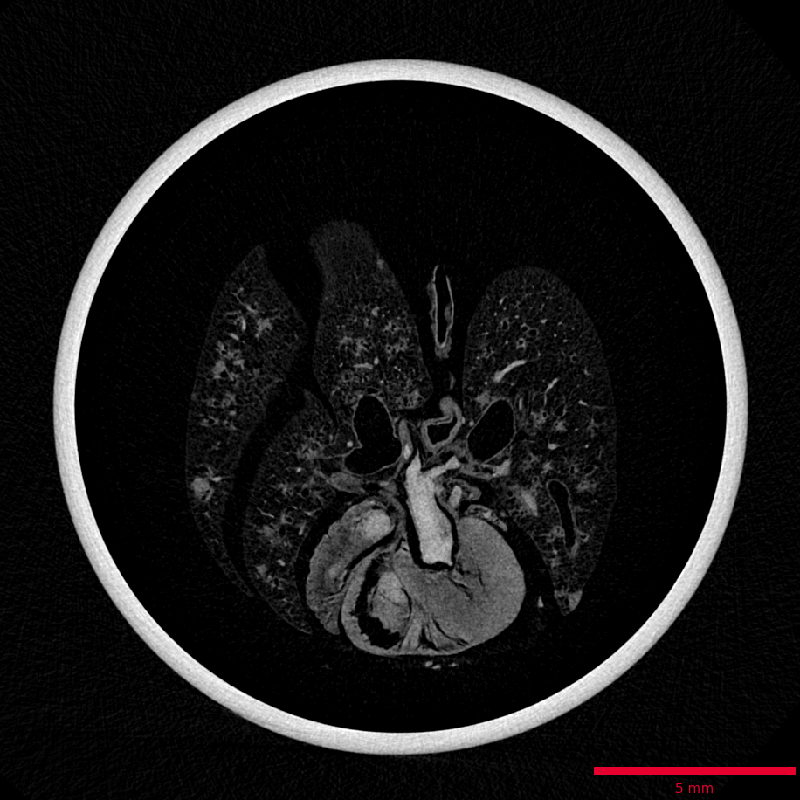
\includegraphics[height=\imageheight]{./movies/scan/reconstructions/KP-TNIKWT02_240_reconstructions_of_556_800_px_100}}
% \end{frame}

% \begin{frame}
% 	\frametitle{Reconstructions}
	\begin{itemize}
		\item Based on hundreds of angular views acquired while the object rotates, a computer synthesizes a stack of virtual cross section slices through the object.
		\item Radon Transformation
		\item Filtered back projection
		\item Fan beam reconstruction
		\item Corrections (beam hardening, etc.)
		\item Writing to stack
	\end{itemize}
\end{frame}

\begin{frame}[allowframebreaks]
	\frametitle{Visualization}
	\begin{tikzpicture}[remember picture,overlay]%
	\node at (current page.center){%
		\mode<beamer>{\animategraphics[autoplay,loop,height=\paperheight,every=\everyframe]{24}{./movies/scan/visualization/lung}{000}{240}}%
		\mode<handout>{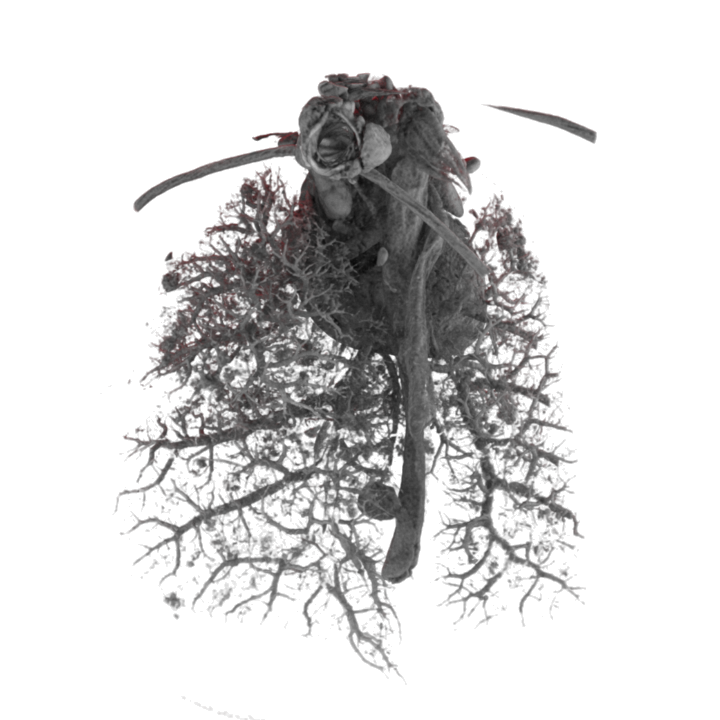
\includegraphics[height=\paperheight]{./movies/scan/visualization/lung000}}%
		};%
	\end{tikzpicture}%
% \end{frame}

% \begin{frame}
% 	\frametitle{Visualization}
		\pagebreak
		\begin{itemize}
			\item Based on the reconstructions, a computer synthesizes a three-dimensional view of the scanned sample
		\end{itemize}
\end{frame}

\subsection{Interaction of x-rays with matter}
\begin{frame}
	\frametitle{X-ray interaction}
	\begin{itemize}
		\item \textquote[\cite{xrayphysics}]{X-rays interact with tissue in 2 main ways: photoelectric effect and Compton scatter.
				To a first approximation, the photoelectric effect contributes to contrast while the Compton effect contributes to noise.
				Both contribute to dose.}
		\begin{itemize}
			\item Photoelectric absorption (\(\tau\)) is strongly dependent on the atomic number \(Z\) of the absorbing material: \(\tau\propto\frac{Z^4}{E^{3.5}}\)
			\note{From \href{https://radiopaedia.org/articles/photoelectric-effect}{Radiopaedia.org}: Therefore if \(Z\) doubles, PEA will increase by a factor of 16 (\(2^4=16\)), and if \(E\) doubles PEA will be reduced by a factor of 11.
				Small changes in \(Z\) and \(E\) can therefore significantly affect PEA.
				This has practical implications in the field of radiation protection and is the reason why materials with a high \(Z\) such as lead (\(Z= 82\)) are useful shielding materials.
				The dependence of PEA on \(Z\) and \(E\) means that it is the major contributor to beam attenuation up to approximately 30 keV when human tissues (\(Z=7.4\)) are irradiated.
				At beam energies above this, the Compton effect predominates.}
		 	\item Compton scattering is one of the principle forms of photon interaction and is directly proportional to the (electron \& physical) density of the material.
		 		It does \emph{not} depend on the atomic number: \(\lambda' - \lambda = \frac{h}{m_e c}\left(1-\cos{\theta}\right)\)
			\note{Where \(\lambda\) is the initial wavelength, \(\lambda'\) is the wavelength after scattering, \(h\) is the Planck constant, \(m_e\) is the electron rest mass, \(c\) is the speed of light, and \(\theta\) is the scattering angle.}
		\end{itemize}
		\item Lowering x-ray energy increases contrast
		\item X-ray penetration decreases exponentially with sample thickness (\cite[\ie Beer-Lamberts law]{wiki:beer-lambert} \(I(t) = I_0 \, e^{-\alpha z}\)
	\end{itemize}
\end{frame}

\begin{frame}
	\frametitle{Composition of biological tissues}
	Tissue: content by mass percentage
	\centering
	\begin{table}%
		\only<1>{%
			\pgfplotstabletypeset[%
				col sep=comma,% the seperator in our .csv file
				display columns/0/.style={string type},%
				% section 3.2 in pgfplotstable manual
				every head row/.style={before row={\toprule}},%
				every row no 0/.style={after row=\midrule},%
				every last row/.style={after row=\bottomrule},%
			]{./tables/tissue-composition.csv}%
		}%
		\only<2>{%
			\pgfplotstabletypeset[%
				col sep=comma,% the seperator in our .csv file
				display columns/0/.style={string type},%
				every head row/.style={before row={\toprule}},%
				every row no 0/.style={after row=\midrule},%
				every last row/.style={after row=\bottomrule},%
				% make certain cells ubRed, based on https://tex.stackexchange.com/a/296914/828
				every row 1 column 2/.style={postproc cell content/.append style={/pgfplots/table/@cell content/.add={\cellcolor{ubRed!61.8}}{}}},%
				every row 1 column 4/.style={postproc cell content/.append style={/pgfplots/table/@cell content/.add={\cellcolor{ubRed!61.8}}{}}},%
				every row 6 column 6/.style={postproc cell content/.append style={/pgfplots/table/@cell content/.add={\cellcolor{ubRed!61.8}}{}}},%
				every row 6 column 10/.style={postproc cell content/.append style={/pgfplots/table/@cell content/.add={\cellcolor{ubRed!61.8}}{}}}%
			]{./tables/tissue-composition.csv}%
		}%
	\end{table}
	\note{Bone, lean tissue, fat and air can be distinguished quite easily}
\end{frame}

\section{Data wrangling by example}
\subsection{Teeth}
\mode<beamer>{%
	\begin{frame}
		\frametitle{Internal morphology of human teeth}
		\begin{tikzpicture}[remember picture,overlay]%
			\node at (current page.center) [shift={(0,-25pt)}]{%
			\animategraphics[autoplay,loop,width=\paperwidth,every=\everyframe]{24}{./movies/tooth045/full/image0}{000}{474}%
				};%
		\end{tikzpicture}%
		Collaboration with \href{https://www.zmk.unibe.ch/}{zmk bern – Zahnmedizinische Kliniken}
		\begin{itemize}
			\item Numbers instead of just pretty images
			\item Segmentation of teeth and root canal
			\item (Unbiased) Characterization
			\item Reproducible and automated image analysis (\href{https://www.python.org/}{\faPython} in \href{https://jupyter.org/}{Jupyter}~\cite{Kluyver2016})
		\end{itemize}
	\end{frame}
}

\begin{frame}
	\frametitle{Internal morphology of human teeth}
	Collaboration with \href{https://www.zmk.unibe.ch/}{zmk bern – Zahnmedizinische Kliniken}\footcite{Haberthuer2021}
	\begin{itemize}
		\item Numbers instead of just pretty images
		\item Segmentation of teeth and root canal
		\item (Unbiased) Characterization
		\item Reproducible and automated image analysis (\href{https://www.python.org/}{\faPython} in \href{https://jupyter.org/}{Jupyter}~\cite{Kluyver2016})
	\end{itemize}
\end{frame}

\begin{frame}
	\frametitle{How?}
	\begin{columns}
		\begin{column}{0.5\linewidth}
			\begin{itemize}
				\item<1-> 104 extracted human permanent mandibular canines
				\item<2-> \uct imaging
				\item<5-> Root canal configuration, according to~\citeauthor{Briseno-Marroquin2015}~\cite{Briseno-Marroquin2015}
				\item<6-> \emph{Reproducible} analysis~\cite{Haberthuer2020a}\onslide<7>{, \eg you can \href{https://mybinder.org/v2/gh/habi/zmk-tooth-cohort/master?filepath=ToothAnalysis.ipynb}{click a button to double-check} or \href{https://nbviewer.jupyter.org/github/habi/zmk-tooth-cohort/blob/master/ToothAnalysis.ipynb}{recalculate the results yourself!}}
			\end{itemize}
		\end{column}
		\begin{column}{0.5\linewidth}
			\only<1|handout:1>{%
				\centering%
				\renewcommand{\imagewidth}{0.75\linewidth}
				\pgfmathsetlength{\imagescale}{\imagewidth/2716}%
				\def\x{1678}% scalebar-x starting at golden ratio of image width of 2716px = 1678
				\def\y{2444}% scalebar-y at 90% of image height of 2716px = 2444
				\begin{tikzpicture}[x=\imagescale,y=-\imagescale]
					\node[anchor=north west, inner sep=0pt, outer sep=0pt] at (0,0) {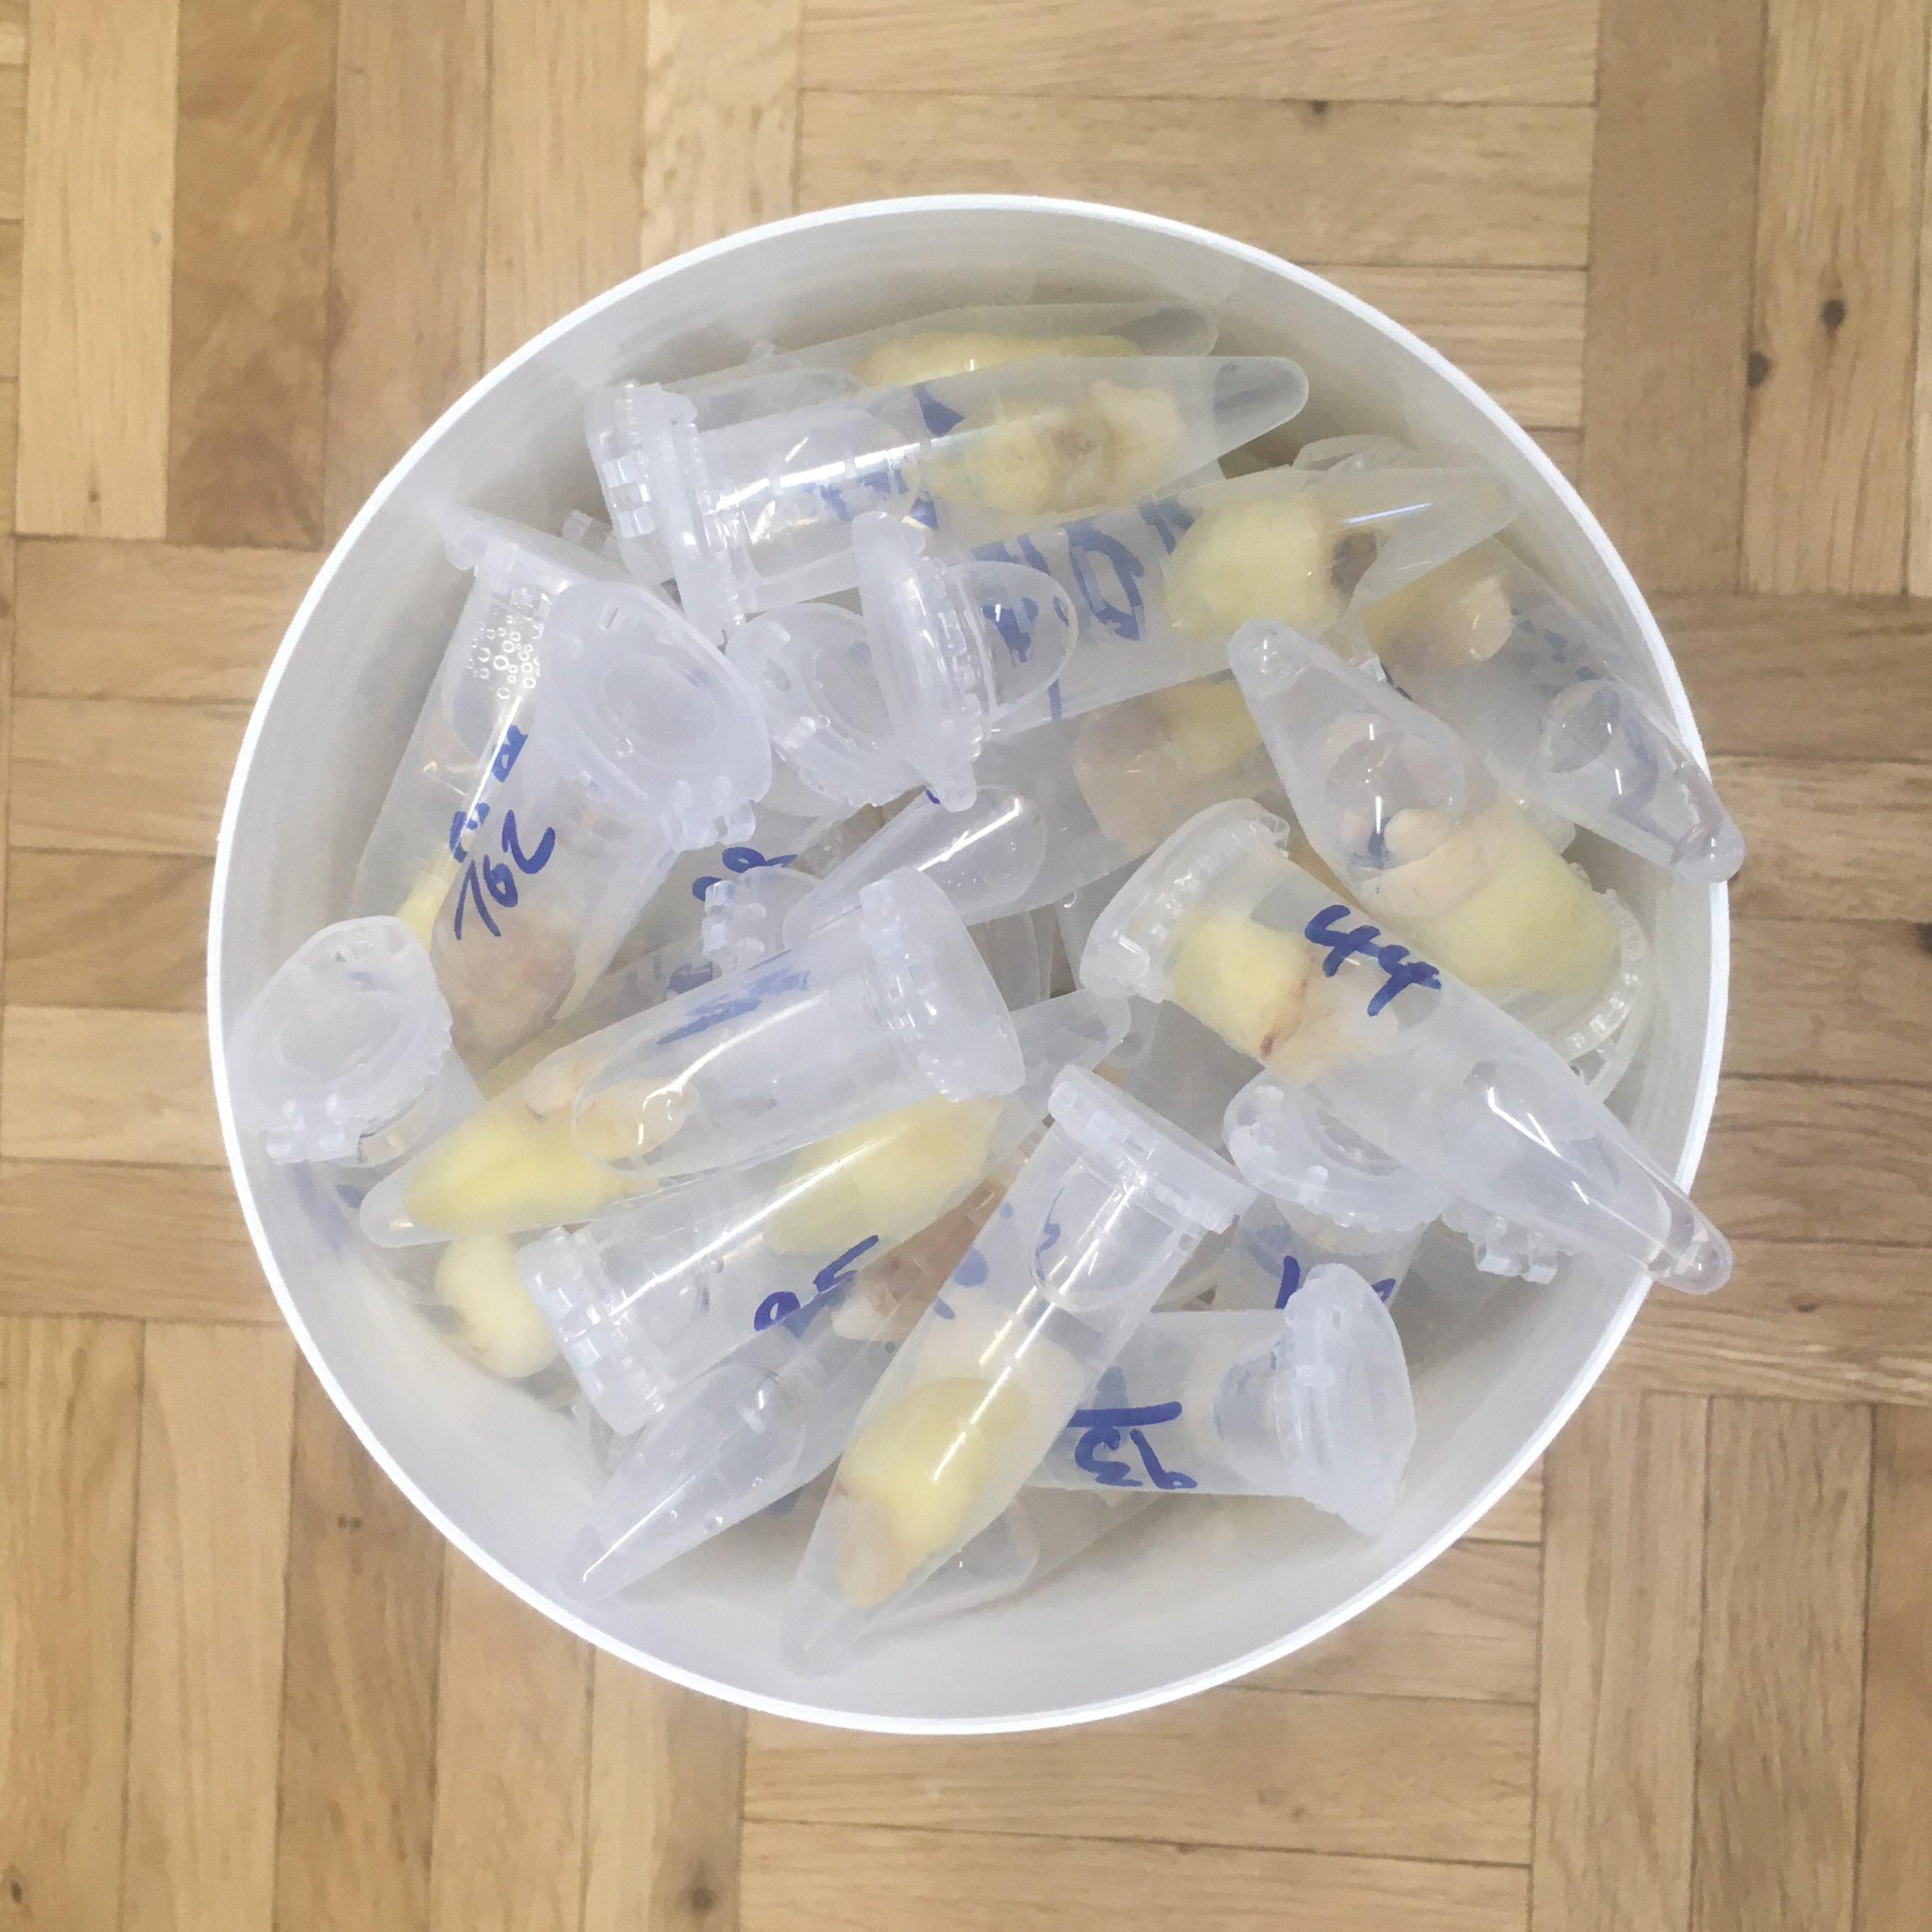
\includegraphics[width=\imagewidth]{./images/bucketofteeth}};
					% 2132.087px = 140.0mm -> 100px = 6566.337um -> 7.615px = 500um, 1.523px = 100um
					%\draw[|-|,blue,thick] (299,1340) -- (2430,1406) node [sloped,midway,above,fill=white,semitransparent,text opacity=1] {\SI{140.0}{\milli\meter} (2132px) TEMPORARY!};
					\draw[|-|,white,thick,shadowed] (\x,\y) -- (\x+761.5,\y) node [midway,above] {\shadowtext{\SI{5}{\centi\meter}}};
				\end{tikzpicture}%
				\renewcommand{\imagewidth}{\columnwidth}
				}%
			\only<2|handout:2>{%
				\centering%
				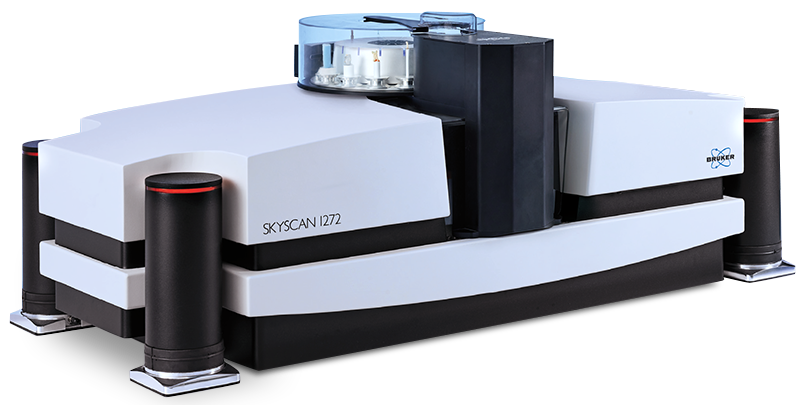
\includegraphics[width=\imagewidth]{./images/1272}%
				\source{bruker.com/skyscan1272}{}%
				}%
			\only<3|handout:3>{%
				\lstinputlisting[linerange={2-4,15-15,17-19,28-30,36-37,40-40,44-44,53-54}]{./logfiles/Tooth045.log}%
				}%
			\only<4|handout:4>{%
				\emph{Sample changer} on the SkyScan 1272\newline
				In total:
				\begin{itemize}
					\item 13 days of \emph{continuous} \uct scanning
					\item \SI{819}{\giga\byte} of raw data\newline\num{230648} TIFF projections
					\item \SI{326}{\giga\byte} data as input for analysis\newline\num{282062} PNG reconstructions
				\end{itemize}
					}%
			\renewcommand{\imagewidth}{\linewidth}%
			\only<5|handout:5>{%
				\centering%
				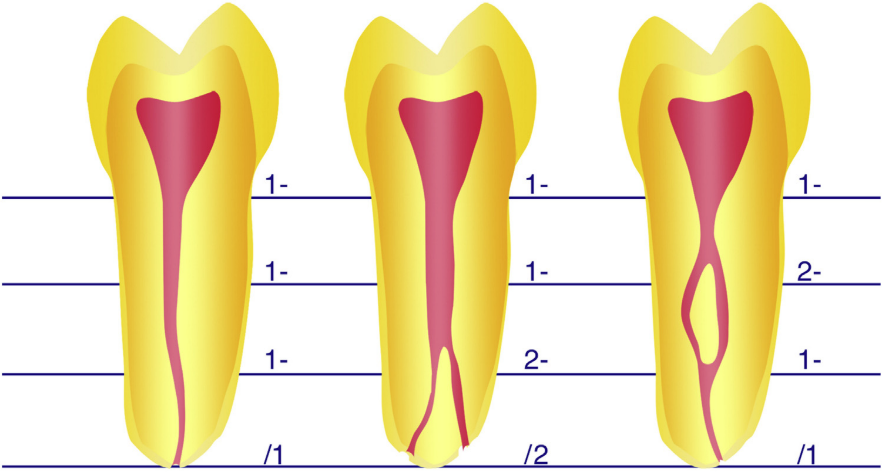
\includegraphics[width=\imagewidth]{./images/briseno}%
				\sourcecite{Briseno-Marroquin2015}{Fig.~2}%
				}%
			\only<6|handout:6>{%
				\centering%
				\mode<beamer>{%
					\animategraphics[loop,autoplay,width=\imagewidth,every=\everyframe]{24}{./movies/coder/coder-}{0}{133}%
					\source{gph.is/2nqkple}{}%
					}%
				\mode<handout>{%
					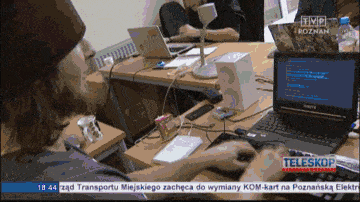
\includegraphics[width=\imagewidth]{./movies/coder/coder-118}%
					\source{gph.is/2nqkple}{}%
					}%
				}%
			\only<7|handout:7>{%
				\centering%
				\href{https://mybinder.org/v2/gh/habi/zmk-tooth-cohort/master?filepath=ToothAnalysis.ipynb}{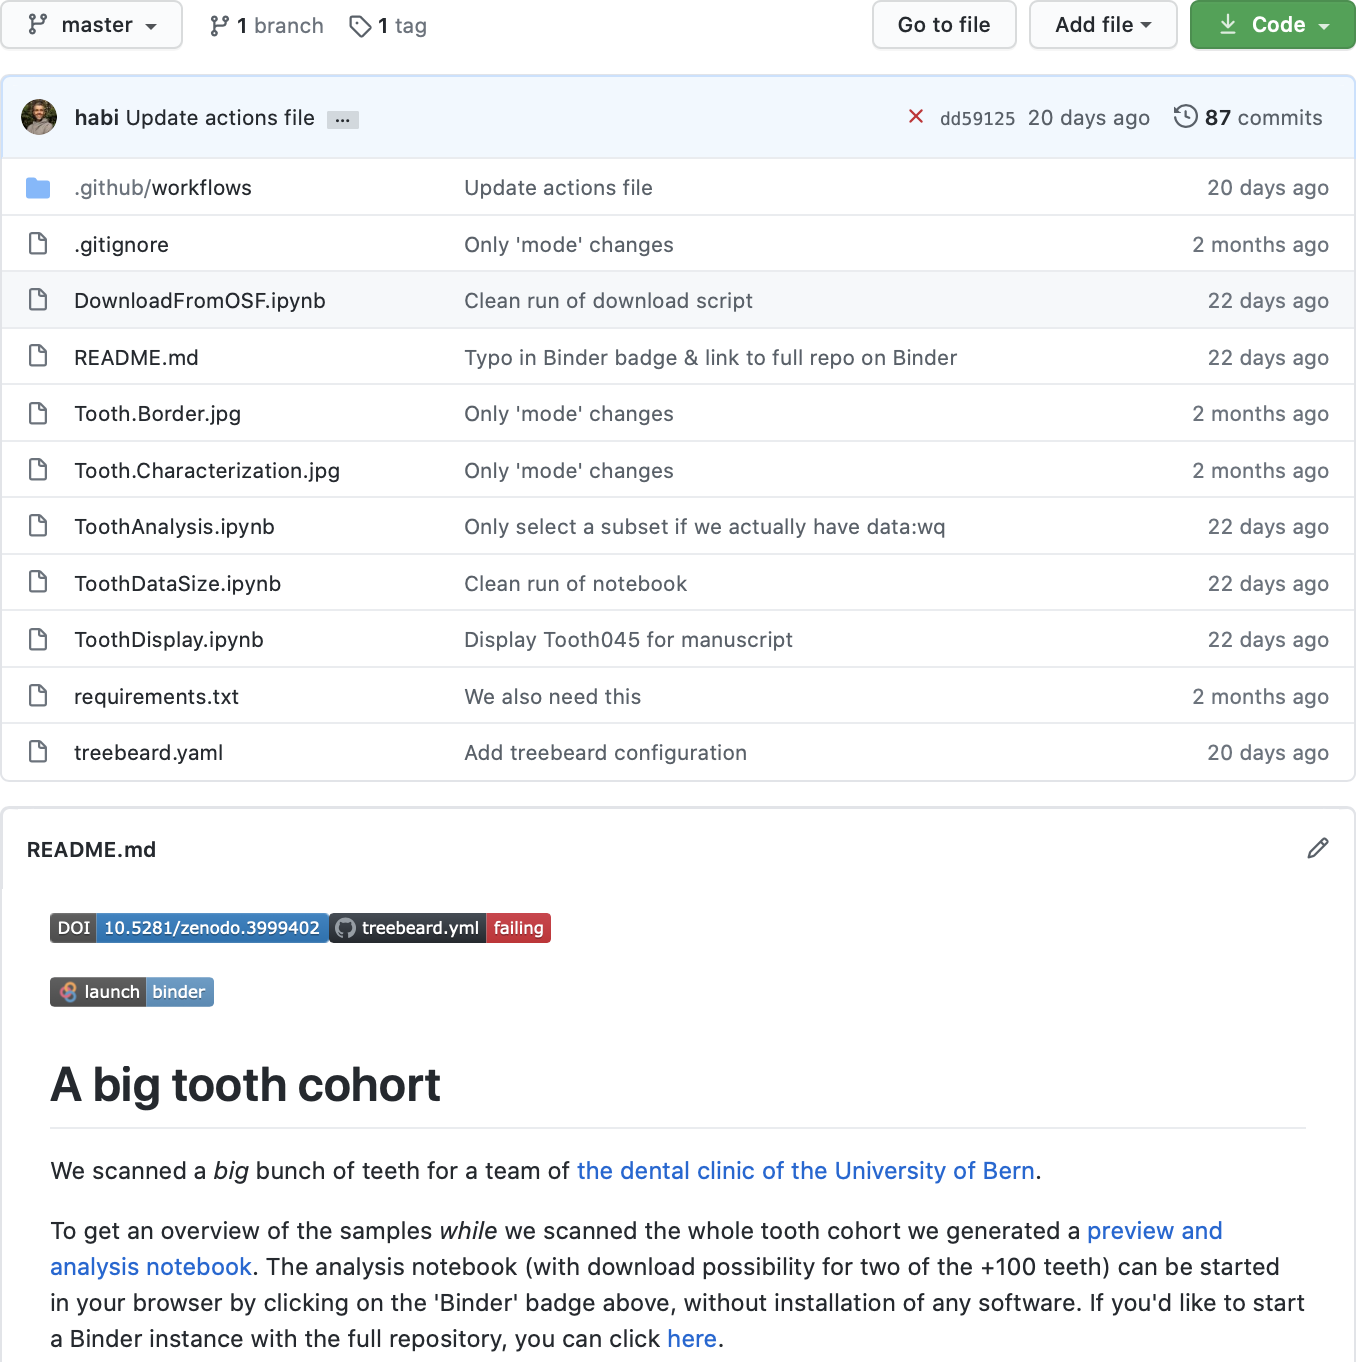
\includegraphics[height=\imageheight]{./images/binder}}%
				}%
		\end{column}
	\end{columns}
\end{frame}

\begin{frame}
	\frametitle{Tooth morphology}
	\begin{tikzpicture}[remember picture,overlay]%
		\node at (current page.center) [shift={(0,-25pt)}]{%
			\only<1|handout:1>{%
				\mode<beamer>{%
					\animategraphics[autoplay,loop,width=\paperwidth,every=\everyframe]{24}{./movies/tooth045/full/image0}{000}{474}%
					}%
				\mode<handout>{%
					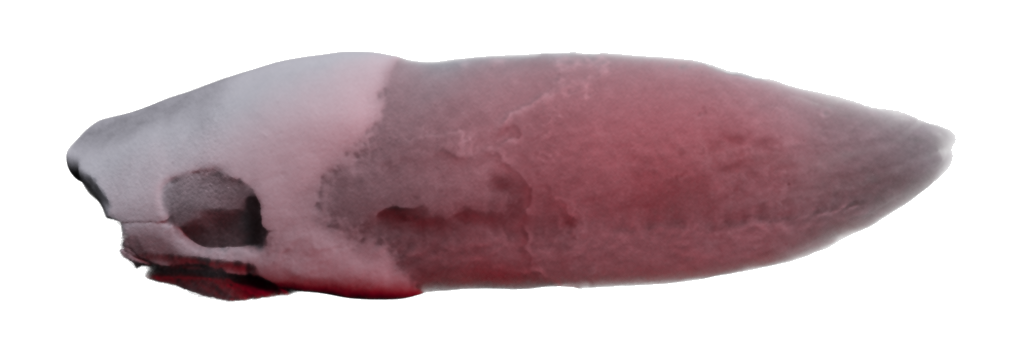
\includegraphics[width=\paperwidth]{./movies/tooth045/full/image0000}%
					}%
				}%
			\only<2|handout:2>{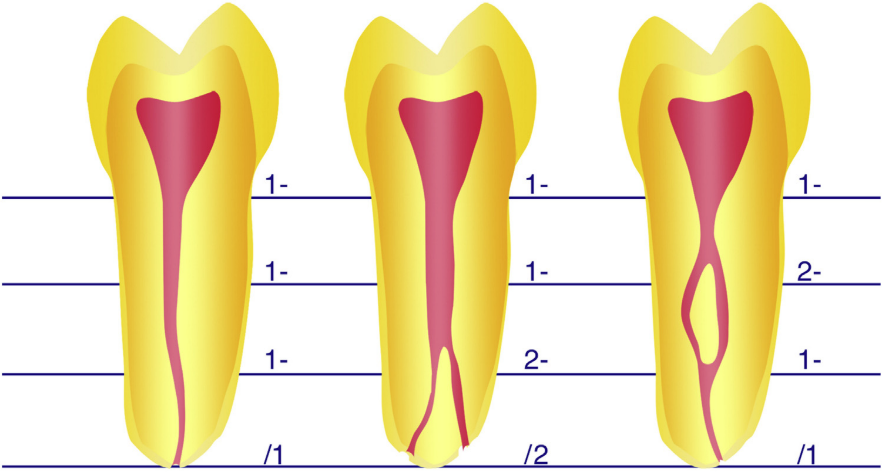
\includegraphics[height=\imageheight]{./images/briseno}\sourcecite{Briseno-Marroquin2015}{Fig.~2}}%
			\only<3|handout:3>{%
				\mode<beamer>{%
					\animategraphics[autoplay,loop,width=\paperwidth,every=\everyframe]{24}{./movies/tooth045/full-slices/image0}{000}{466}%
					}%
				\mode<handout>{%
					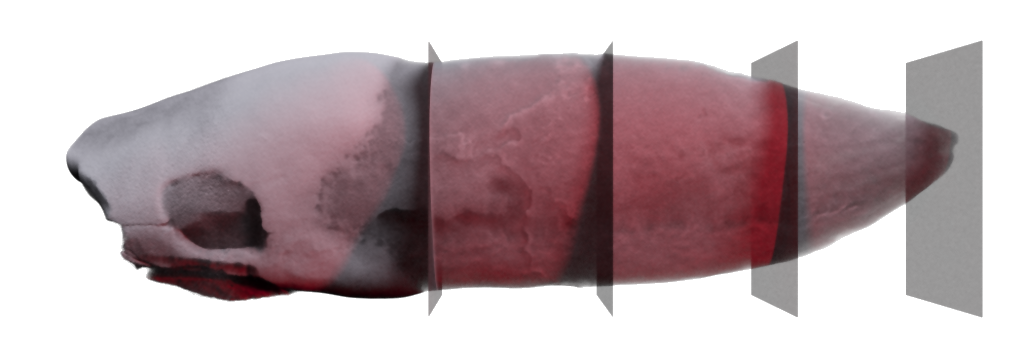
\includegraphics[width=\paperwidth]{./movies/tooth045/full-slices/image0000}%
					}%
				}%
			};%
	\end{tikzpicture}%
\end{frame}

\begin{frame}
	\frametitle{Extraction of root canal space}
	\begin{tikzpicture}[remember picture,overlay]%
	\node at (current page.center) [shift={(0,-25pt)}]{%
		\only<1|handout:0>{%
			\mode<beamer>{%
				\animategraphics[autoplay,loop,width=\paperwidth,every=\everyframe]{24}{./movies/tooth045/transparent-slices/image0}{000}{473}%
				}%
			\mode<handout>{%
				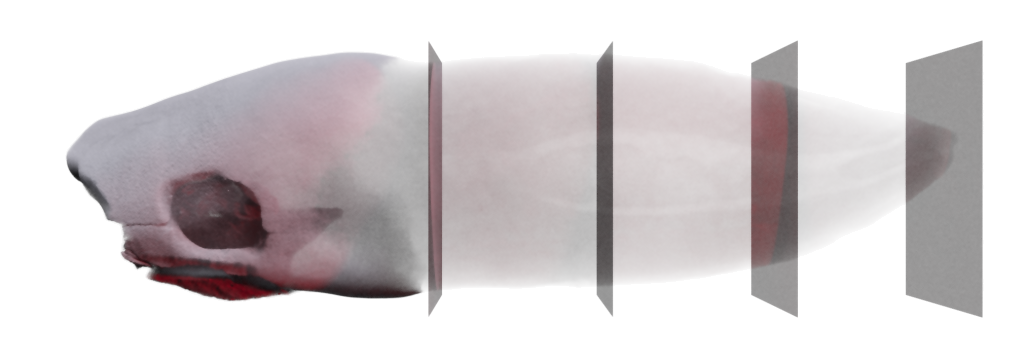
\includegraphics[width=\paperwidth]{./movies/tooth045/transparent-slices/image0000}%
				}%
			}%
		\only<2|handout:1>{%
			\mode<beamer>{%
				\animategraphics[autoplay,loop,width=\paperwidth,every=\everyframe]{24}{./movies/tooth045/transparent-slices-rcs/image0}{000}{457}%
				}%
			\mode<handout>{%
				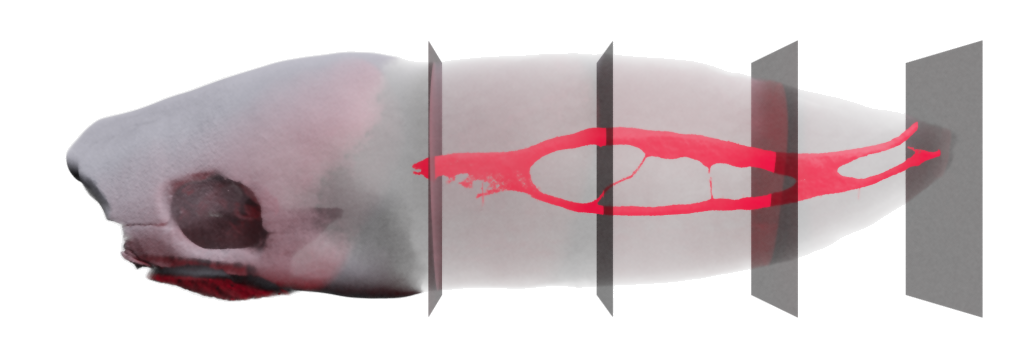
\includegraphics[width=\paperwidth]{./movies/tooth045/transparent-slices-rcs/image0000}%
				}%
			}%
		\only<3|handout:0>{%
			\mode<beamer>{%
				\animategraphics[autoplay,loop,width=\paperwidth,every=\everyframe]{24}{./movies/tooth045/rcs/image0}{000}{413}%
				}%
			\mode<handout>{%
				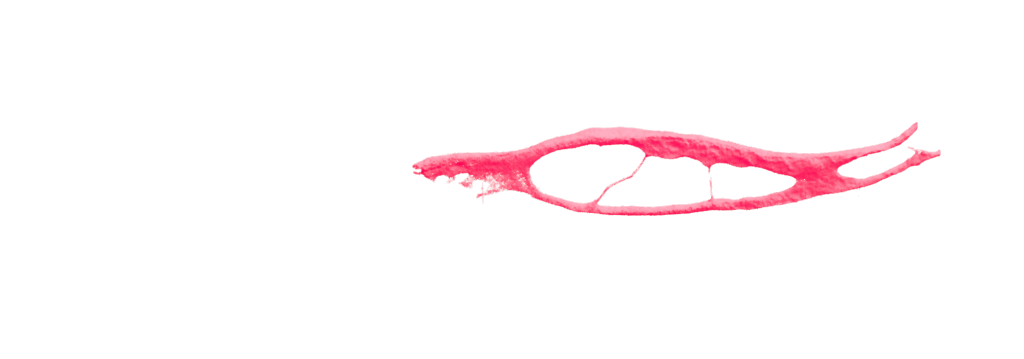
\includegraphics[width=\paperwidth]{./movies/tooth045/rcs/image0000}%
				}%
			}%
		};%
	\end{tikzpicture}%
\end{frame}

\subsection{Fish I}
\begin{frame}
	\frametitle{Data wrangling by example: Cichlids}
	\begin{columns}
		\begin{column}{0.49\linewidth}
			\begin{itemize}
				\item 372 tomographic scans of 133 different Cichlids, from \SIrange{6}{18}{\centi\meter}
				\item \SI{9.8}{\tera\byte} of projection images, \SI{1.5}{\tera\byte} of reconstructions
				\item Reproducible and automated dataset wrangling, checking and image analysis (\href{https://www.python.org/}{\faPython} in \href{https://jupyter.org/}{Jupyter}~\cite{Kluyver2016})
			\end{itemize}
		\end{column}
		\begin{column}{0.49\linewidth}
			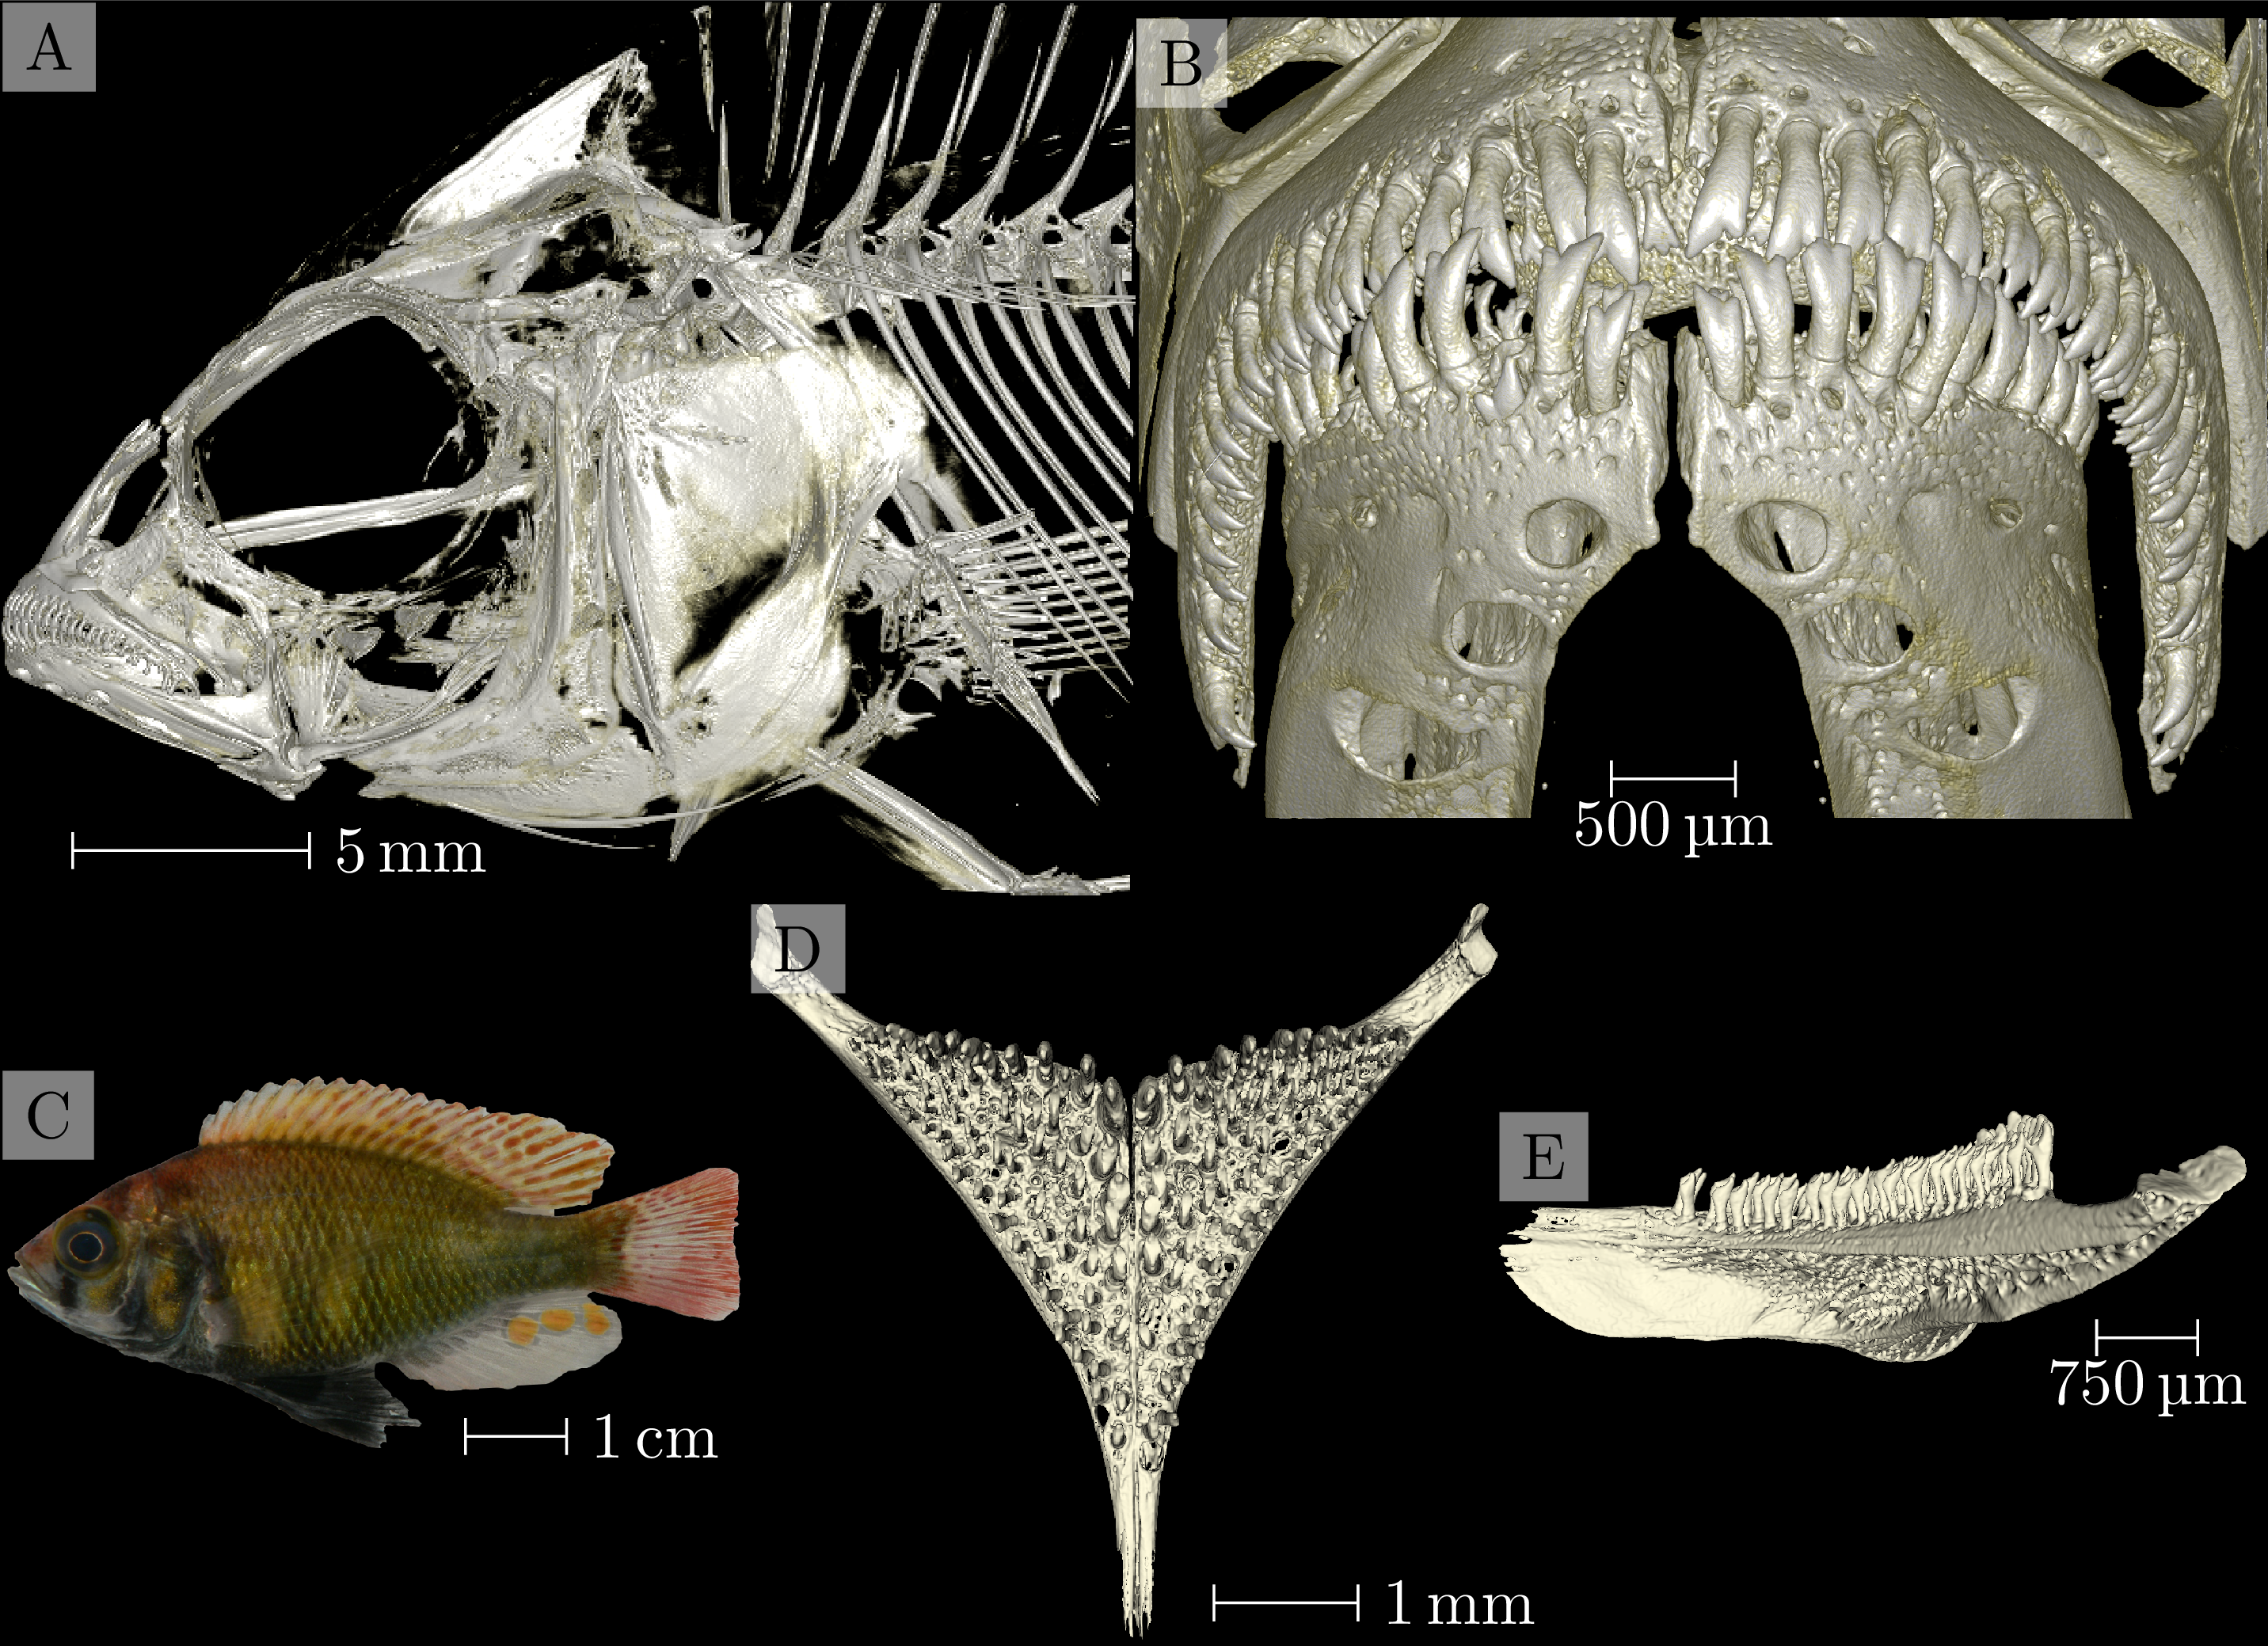
\includegraphics[width=\imagewidth]{./images/cichlids/104016}%
			\sourcecite{Haberthuer2023}{Fig.~1}%
		\end{column}
	\end{columns}
\end{frame}

\begin{frame}
	\frametitle{Data wrangling by example: Cichlids}
	\centering
	\includegraphics<1>[height=\imageheight]{./images/cichlids/Otolither_104016_head_01_Overview}%
	\includegraphics<2>[height=\imageheight]{./images/cichlids/Otolither_104016_head_02_GrayValues}%
	\includegraphics<3>[height=\imageheight]{./images/cichlids/Otolither_104016_head_03_GrayValuesRegion}%
	\includegraphics<4>[height=\imageheight]{./images/cichlids/Otolither_104016_head_04_GrayValuesSmoothed}%
	\includegraphics<5>[height=\imageheight]{./images/cichlids/Otolither_104016_head_05_Peaks}%
	\includegraphics<6>[height=\imageheight]{./images/cichlids/Otolither_104016_head_06_Peaks_All}%
	\includegraphics<7>[height=\imageheight]{./images/cichlids/Otolither_104016_head_07_ExtractedRegions}%
	\includegraphics<8>[height=\imageheight]{./images/cichlids/Otolither_104016_head_08_ExtractedRegionsMIPs}%
	\includegraphics<9>[height=\imageheight]{./images/cichlids/Otolither_104016_head_09_ExtractedOtolithMasked}%
	\only<10>{\href{https://htmlpreview.github.io/?https://github.com/habi/EAWAG-manuscript/blob/main/content/data/104016_Enterochromis_I_cinctus_St_E.head.rec.Otolith.Region.3D.html}{Exported 3D view}}%
\end{frame}

\section{\emph{Take-home} message}
\begin{frame}
	\begin{itemize}
		\item Ask us anything!
		\item Let's do most of this in the \emph{Hands-on} sessions!
	\end{itemize}
\end{frame}

\begin{frame}[allowframebreaks]
	\frametitle{References}%
	\renewcommand*{\bibfont}{\scriptsize}%
	\setbeamertemplate{bibliography item}{\insertbiblabel}%
	\printbibliography%
\end{frame}

\end{document}
